\nxSections{Hypotenuse}{2}

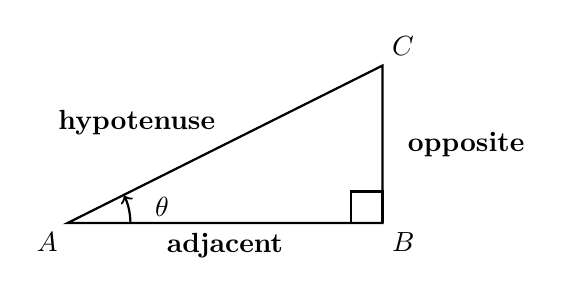
\begin{tikzpicture}[scale=2]
  % Triangle
  \coordinate (A) at (0,0);
  \coordinate (B) at (2,0);
  \coordinate (C) at (2,1);
  \draw[thick] (A) -- (B) -- (C) -- cycle;

  % Right angle glyph
  \draw[thick] (B) -- ++(0,0.2) -- ++(-0.2,0) -- ++(0,-0.2);

  % Labels
  \node[below left] at (A) {\( A \)};
  \node[below right] at (B) {\( B \)};
  \node[above right] at (C) {\( C \)};
  \node at (1,0) [below] {\textbf{adjacent}};
  \node at (2.1,0.5) [right] {\textbf{opposite}};
  \node at (1,0.5) [above left] {\textbf{hypotenuse}};

  % Angle theta
  \draw[->, thick] (0.4,0) arc[start angle=0,end angle=26,radius=0.4];
  \node at (0.6,0.1) {\( \theta \)};
\end{tikzpicture}

\begin{empheq}[box=\nxWarningMathBox]{align}
  \sin\theta &= \frac{\text{opposite}}{\text{hypotenuse}} \\
  \cos\theta &= \frac{\text{adjacent}}{\text{hypotenuse}} \\
  \tan\theta &= \frac{\text{opposite}}{\text{adjacent}}
\end{empheq}

\begin{empheq}[box=\nxWarningMathBox]{align*}
  \text{Hypotenuse} &= \text{always opposite the right angle} \\
  \text{Opposite} &= \text{side across from the angle you're analyzing} \\
  \text{Adjacent} &= \text{side next to the angle (not hypotenuse)}
\end{empheq}

\nxSections{Standard Position of an Angle}{2}
\begin{empheq}[box=\nxWarningMathBox]{align*}
  \text{Vertex} &= \text{Origin} \ (0,0) \\
  \text{Initial Side} &= \text{Positive } x\text{-axis} \\
  \text{Terminal Side} &= \text{Rotated ray from origin}
\end{empheq}

\begin{empheq}[box=\nxWarningMathBox]{align*}
  \theta &= 60^\circ \quad \text{(Quadrant I)} \\
  \theta &= 150^\circ \quad \text{(Quadrant II)} \\
  \theta &= -45^\circ \quad \text{(Clockwise)}
\end{empheq}


\nxSections{Hypotenuse}{2}
The hypotenuse is the longest side of a right-angled triangle — the side opposite the right angle. It’s the sacred diagonal that connects the two legs and completes the triangle’s invocation.
\newpage

\nxSections{Pythagorean Theorem (Right Triangle Only)}{3}
\begin{empheq}[box=\nxWarningMathBox]{align}
  c &= \sqrt{a^2 + b^2}
\end{empheq}

\begin{tikzpicture}[scale=1.5]
  \coordinate (A) at (0,0);
  \coordinate (B) at (3,0);
  \coordinate (C) at (3,4);
  \draw[thick] (A) -- (B) -- (C) -- cycle;
  \draw (B) -- ++(0,0.4) -- ++(-0.4,0) -- ++(0,-0.4);

  \node[below left] at (A) {\( A \)};
  \node[below right] at (B) {\( B \)};
  \node[above right] at (C) {\( C \)};
  \node at (1.5,0) [below] {\( a = 3 \)};
  \node at (3.2,2) [right] {\( b = 4 \)};
  \node at (1.5,2.2) [above left] {\( c = ? \)};
\end{tikzpicture}
\bigskip

\begin{empheq}[box=\nxSuccessMathBox]{align*}
  c &= \sqrt{3^2 + 4^2} = \sqrt{9 + 16} = \sqrt{25} = 5
\end{empheq}

\newpage




\nxSections{Trigonometric Ratios}{3}
\begin{empheq}[box=\nxWarningMathBox]{align}
  c &= \sqrt{a^2 + b^2}
\end{empheq}
\bigskip

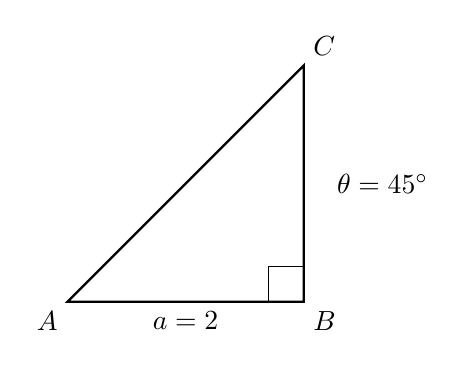
\begin{tikzpicture}[scale=1.5]
  \coordinate (A) at (0,0);
  \coordinate (B) at (2,0);
  \coordinate (C) at (2,2);
  \draw[thick] (A) -- (B) -- (C) -- cycle;
  \draw (B) -- ++(0,0.3) -- ++(-0.3,0) -- ++(0,-0.3);

  \node[below left] at (A) {\( A \)};
  \node[below right] at (B) {\( B \)};
  \node[above right] at (C) {\( C \)};
  \node at (1,0) [below] {\( a = 2 \)};
  \node at (2.2,1) [right] {\( \theta = 45^\circ \)};
\end{tikzpicture}
\bigskip

\begin{empheq}[box=\nxSuccessMathBox]{align*}
  c &= \frac{a}{\cos\theta} = \frac{2}{\cos 45^\circ} = \frac{2}{\frac{\sqrt{2}}{2}} = 2\sqrt{2}
\end{empheq}
\newpage



\nxSections{Law of Cosines (Any Triangle)}{3}
\begin{empheq}[box=\nxWarningMathBox]{align}
  c^2 &= a^2 + b^2 - 2ab\cos\gamma
\end{empheq}
\bigskip

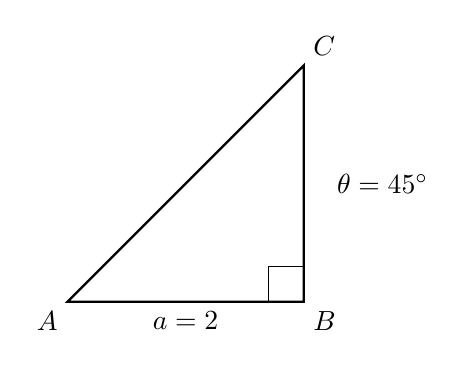
\begin{tikzpicture}[scale=1.5]
  \coordinate (A) at (0,0);
  \coordinate (B) at (2,0);
  \coordinate (C) at (2,2);
  \draw[thick] (A) -- (B) -- (C) -- cycle;
  \draw (B) -- ++(0,0.3) -- ++(-0.3,0) -- ++(0,-0.3);

  \node[below left] at (A) {\( A \)};
  \node[below right] at (B) {\( B \)};
  \node[above right] at (C) {\( C \)};
  \node at (1,0) [below] {\( a = 2 \)};
  \node at (2.2,1) [right] {\( \theta = 45^\circ \)};
\end{tikzpicture}
\bigskip

\begin{empheq}[box=\nxSuccessMathBox]{align*}
  c &= \frac{a}{\cos\theta} = \frac{2}{\cos 45^\circ} = \frac{2}{\frac{\sqrt{2}}{2}} = 2\sqrt{2}
\end{empheq}
\newpage


\nxSections{Coordinate Geometry (Distance Formula)}{3}

\begin{empheq}[box=\nxWarningMathBox]{align}
  c &= \sqrt{(x_2 - x_1)^2 + (y_2 - y_1)^2}
\end{empheq}
\bigskip

\begin{tikzpicture}[scale=1.5]
  \coordinate (P) at (0,0);
  \coordinate (Q) at (2,1.5);
  \draw[thick] (P) -- (Q) node[midway, above left] {\( c = ? \)};
  \draw[dashed] (P) -- (2,0) -- (Q);

  \node[below left] at (P) {\( (x_1, y_1) = (0,0) \)};
  \node[above right] at (Q) {\( (x_2, y_2) = (2,1.5) \)};
\end{tikzpicture}
\bigskip

\begin{empheq}[box=\nxSuccessMathBox]{align*}
  c &= \sqrt{(2 - 0)^2 + (1.5 - 0)^2} \\
    &= \sqrt{4 + 2.25} = \sqrt{6.25} = 2.5
\end{empheq}
\newpage

